% One-pager on Figure 3 of Experiment 4 (layers and range): the measurement, how the figure is built, what it can and cannot show.
% Run results/20261024-000548_exp4ctrl; figure from ../exp4/onepager_figures.py (fig_layers, retention).
% Numbers: exp4/LOG.md; "without the four heads" and the CIs were recomputed from controlled.npz. Build (from this folder): pdflatex exp4_fig3_onepager.tex
\documentclass[10pt]{article}
\usepackage[letterpaper,hmargin=0.5in,vmargin=0.3in]{geometry}
\usepackage[T1]{fontenc}
\usepackage[scaled=0.92]{helvet}
\renewcommand{\familydefault}{\sfdefault}
\usepackage{microtype}
\usepackage{amsmath,amssymb}
\usepackage{xcolor}
\usepackage{graphicx}
\usepackage{enumitem}
\usepackage[hidelinks]{hyperref}
\setlength{\parindent}{0pt}
\setlength{\parskip}{2pt}
\setlist{nosep,leftmargin=1.5em,itemsep=1.5pt}
\definecolor{cblue}{HTML}{2A78D6}
\definecolor{corange}{HTML}{EB6834}
\definecolor{ink2}{HTML}{52514E}
\definecolor{muted}{HTML}{898781}
\definecolor{axis}{HTML}{C3C2B7}
\definecolor{plane}{HTML}{F4F3EF}
\definecolor{wordbg}{HTML}{DCEAFB}

% token chips: \tb BOS, \tk random filler, \tw inserted country, \tq final token (the query whose attention is read)
\newcommand{\chip}[3]{{\setlength{\fboxsep}{1pt}\setlength{\fboxrule}{0.4pt}\fcolorbox{#1}{#2}{\strut\ttfamily\footnotesize #3}}\hspace{0.8pt}}
\newcommand{\tb}{\chip{ink2}{ink2}{\color{white}BOS}}
\newcommand{\tk}[1]{\chip{axis}{white}{\color{muted}#1}}
\newcommand{\tw}[1]{\chip{cblue}{wordbg}{#1}}
\newcommand{\tq}[1]{\chip{corange}{white}{\bfseries #1}}
\newcommand{\gap}[1]{{\color{muted}\footnotesize\,\dots\,#1\,\dots\,}}
\newcommand{\ex}[1]{\leavevmode\makebox[1.45cm][l]{\color{ink2}\small\bfseries #1}}
\newcommand{\head}[2]{\par{\large\bfseries #1}\hfill{\color{muted}\footnotesize #2}\\[-3pt]\rule{\linewidth}{0.5pt}\par}

\begin{document}

\head{1\textperiodcentered\ Set up}{}
\small
{\linespread{1.18}\selectfont
\begin{enumerate}[label=\textbf{(\alph*)},itemsep=6pt]
\item \textbf{Attention weight.} Each head in each layer gives the final token $T$ a probability distribution over every earlier
  position, BOS included, so the weights sum to 1 and attention gained at one position is lost at others. $a$ is the share of one
  head's lookup that lands on position $\tau$.
\item \textbf{Intervention.} A row is BOS plus 32 random tokens with no repeats. $T$ (position 32) is the query and is never edited.
  For each $\tau = 1\ldots31$, one of 11 countries replaces the token at $\tau$ and nothing else changes. The unedited row is the
  control, so any change in $a$ is caused by the token at $\tau$, through its key or through how earlier layers changed $T$'s query.\\[4pt]
  \ex{control}\tb\tk{she}\tk{sc}\gap{27 random tokens}\tk{age}\tk{dis}\tq{ious}\hspace{1.2em}%
  \ex{country}\tb\tk{she}\tk{sc}\gap{27 random tokens}\tw{France}\tk{dis}\tq{ious}\hspace{0.5em}{\footnotesize\color{muted}($\tau$ = 30, $d$ = 2)}
\item \textbf{The number.} $\Delta = a_{\text{country at }\tau} - a_{\text{control at }\tau}$, for each head and each distance
  $d = 32-\tau$ ($d=1$ is the adjacent slot), averaged over the 11 countries so each row counts once.
\item \textbf{Scale.} 200 rows per filler type (common: token ids 256--999, rare: 1000--39999) $\times$ 11 countries $\times$ 31
  positions, 68,200 forward passes per filler type. The result is an array $x[\text{row}, d, \text{layer}, \text{head}]$ of size
  $200 \times 31 \times 12 \times 12$.
\par
\end{enumerate}}
{\setlength{\abovedisplayskip}{2pt}\setlength{\belowdisplayskip}{2pt}%
\setlength{\abovedisplayshortskip}{2pt}\setlength{\belowdisplayshortskip}{2pt}
\begin{align*}
x[r,d,\ell,h] &= \frac{1}{11}\sum_{c=1}^{11} a^{(c)}_{r,\ell,h}(\tau) \;-\; a^{0}_{r,\ell,h}(\tau)
  \;=\; \mathbb{E}_{c}\!\left[a^{(c)}_{r,\ell,h}(\tau)\right] - a^{0}_{r,\ell,h}(\tau), \qquad \tau = 32 - d\\
M_\ell(d) &= \frac{1}{200}\sum_{r=1}^{200}\;\frac{1}{12}\sum_{h=1}^{12} x[r,d,\ell,h]
  \;=\; \mathbb{E}_{r,\,h}\!\left[x[r,d,\ell,h]\right]
\end{align*}}%
\noindent Let\par\nopagebreak
{\renewcommand{\arraystretch}{1.3}%
\begin{tabular}{@{\hspace{2em}}l@{\hspace{0.9em}}p{0.68\linewidth}@{}}
$r\in\{1,\dots,200\}$ & be the row index, \\
$c\in\{1,\dots,11\}$ & be the country index, \\
$\ell\in\{0,\dots,11\}$ & be the layer index, \\
$h\in\{1,\dots,12\}$ & be the head index, \\
$d\in\{1,\dots,31\}$ & be the distance, \\
$\tau=32-d$ & be the position of the inserted country, \\
$a^{(c)}_{r,\ell,h}(\tau)$ & be the attention from $T$ to position $\tau$ in row $r$, layer $\ell$, head $h$, with country $c$ at $\tau$, \\
$a^{0}_{r,\ell,h}(\tau)$ & be the same quantity in the control row, \\
$\mathbb{E}_c$ & be the uniform mean over the 11 countries, \\
$\mathbb{E}_r$ & be the uniform mean over the 200 rows, \\
$\mathbb{E}_h$ & be the uniform mean over the 12 heads of layer $\ell$, and \\
$M_\ell(d)$ & be the value of one heatmap cell (layer $\ell$, distance $d$), computed separately for each filler type.
\end{tabular}}

\vspace{12pt}
\head{2\textperiodcentered\ Figures}{no model run: saved arrays only}
{\centering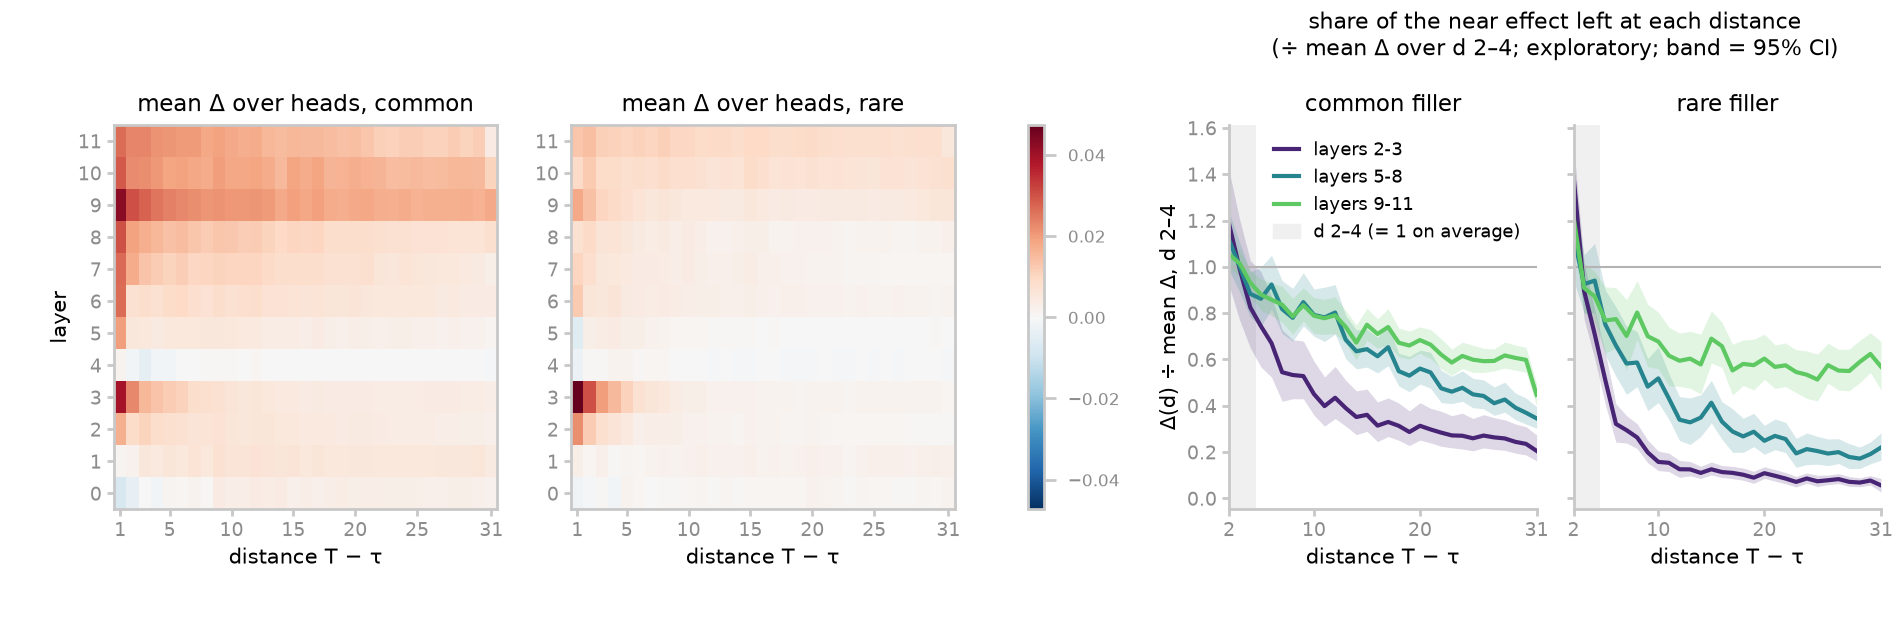
\includegraphics[width=\linewidth]{exp4_layers.png}\par}
\begin{itemize}
\item \textbf{Right.} Let $\mathcal N=\{2,3,4\}$ be the near distances ($d=1$ is left out) and
  $G\in\{\{2,3\},\{5,\dots,8\},\{9,10,11\}\}$ a layer group. Each curve is, for $d = 2,\dots,31$,
  {\setlength{\abovedisplayskip}{2pt}\setlength{\belowdisplayskip}{2pt}%
  \[
  \text{share}_G(d) = \frac{\mathbb{E}_{\ell\in G}\,M_\ell(d)}{\mathbb{E}_{\ell\in G,\,d'\in\mathcal N}\,M_\ell(d')}
  \]}%
  \begin{itemize}
  \item \textbf{Layers 2--3 (24 heads).} The steepest fall: 0.49 (common) and 0.22 (rare) of the near effect over $d$ = 5--15, then 0.28 and 0.09 over $d$ = 16--31.
  \item \textbf{Layers 5--8 (48 heads).} 0.78 (common) and 0.49 (rare) over $d$ = 5--15, then 0.48 and 0.23 over $d$ = 16--31.
  \item \textbf{Layers 9--11 (36 heads).} The flattest: 0.79 and 0.68 over $d$ = 5--15, then 0.63 and 0.57 over $d$ = 16--31. With common filler it is no different from layers 5--8 over $d$ = 5--15 (0.79 vs 0.78).
  \end{itemize}
\end{itemize}

\end{document}
